\chapter{Trustable Oracles }\label{chap:chap5}

\section*{}

At this point, a definition, of what trust in an oracle is, seems appropriate. Trust has a lot of meanings, depending on the needs of all the parties involved. I will model several levels of trust and the requirements and fallacies of each model as well as its application and drawbacks.

Starting from an absolute trust scenario, in this model, the end user, being the smart contract which receives information provided by the oracle, has complete assurances from both the veracity of the data provided by the data source, as well as, undeniable proof that the oracle did not tamper with the relayed information. This scenario points out two main points of failure, either maliciously or unintentionally.

The first component which can be faulty or compromised is the data source. Assuring that the information provided is correct does not have a straightforward answer. What correct means is open to interpretation. For example, if the data source is an IoT sensor, which is prone to failures, being correct is relative. The sensor needs to be perfectly calibrated and accurate. In this case, using several sensors and averaging its values or removing outliers would solve its correctness. Another example could be an API that returns the current value of the EUR in USD. In this scenario, a party that would benefit from a higher conversion than the real one could coerce or attack the data-source into providing a favourable value. The answer here can also be using several data sources. Another solution would be to use a highly trusted entity such as the European Central Bank (ECB) which can be a lot harder to coerce or attack and having a signature from the ECB that backs the provided data. Choosing what type of data-source to use has a huge impact on the trust fullness of the provided data not to mention architecture centralization when using a source such as the ECB. All in all, the end user will have to understand the requirements and level of trust necessary.

The second, and most relevant for analysis, is the oracle service used. Oracles are a necessary part of the process since the other option would be having the data providers adapting to the blockchain which does not seem to be a realistic option at the moment. Therefore we must trust an oracle or a group of oracles. Two main options are available, either trusting a third-party oracle or self-deploying an oracle. In the first scenario, three variables take part in the level of trust. Firstly he third-party oracle, if paid for, has the monetary incentive to be honest, since a bad record of dishonesty would have the service losing credibility and therefore clients. Secondly, by using proofs the oracle can establish its legitimacy, as long as, the proofs can undoubtedly be trusted and verifiable by the smart contract, I will later analyse in depth this issue. Finally, oracle execution transparency by using open-source code and having means for being audited. Additionally, to guaranteeing single oracle integrity, it may be in the interest of the user to use several oracles either to provide service availability or to increase trust by combining the result from different oracle services.


\section{Oracle Architectures}

Having analysed what trust means, it is evident that no short definition is appropriate and that it depends on the stakeholder beliefs. Hence, several architectural models for what a trustable system arise. Varying in decentralization and complexity. Each model satisfies different requirements, such as performance, security and decentralization.
In this section, I will describe several possible architectures and point out use cases and compromises for each model.

\subsection{Oracle as a Service w/ Single Data Feed.}\label{OaaSwSingleDataFeed}

\subsubsection{Context}
Connecting smart contracts with information provided by data-feeds, which do not, by themselves, input the required information on the blockchain requires the use of a trusted oracle. Developing and maintaining a oracle may be prohibitive in terms of cost and desired time to market. Outsourcing such service would be desirable in this context, it may not be in the interest of the company to specialize in the secure development of oracles.

\subsubsection{Example}



\subsubsection{Problem}
How can a non-blockchain company keep up with the fast pace of industry while maintaining trust in its services? It is critical to be able to quickly build a smart contract and connect it with the needed information. How can a company do so, without allocating human resources into to the development of yet another service and simply focus on its business logic?

\subsubsection{Forces}

\begin{itemize}
  \item \textbf{Fast time to market} - Not having to assemble a team or allocate resources into a developing a new product which will only serve as component of the main product being developed.
  \item \textbf{Keeping trust standards} - The company focus is not the development and securement of the oracle service and may not have enough resources to keep the oracle as secure and reliable as the underlying blockchain.
\end{itemize}


\subsubsection{Solution}
Oracle as a service, come as a quick and efficient solution for fast moving companies and individuals. Providing easy integration between a smart contract and a data-feed by means of specific function calls and/or libraries. Theses services are per-request fee-based and can be cheaper comparing to assemblying a team dedicated to the development and maintainance of an oracle. The fee-based system increases the trust in the service as being honest is crucial to their business model. Additionally, this services usally provide authenticity proofs which serve as another layer of trust in the service. In the chapter \ref{chap:chap4} I deep dive on the subject of the proofs.

\begin{figure*}[t]
  \begin{center}
    \leavevmode
    \includegraphics[width=0.5\textwidth]{figures/oraclearch1.jpg}
    \caption{Oracle as a Service w/ Single Data Feed.}
    \label{fig:/figures/paper-screening}
  \end{center}
\end{figure*}

\subsubsection{Example Resolved}


\subsubsection{Resulting Context}
%% FIXME: o resulting context muitas vezes foca-se nos "quality attributes" (e.g., trust, reliability, resilience, cost) que são característica da solução. ao ler esta secção fico a achar que estas características estão de facto aqui descritas, mas às vezes é preciso ler nas entrelinhas quais são. uma forma de as tornar mais visíveis é estruturar este texto como bullet points (um ponto por quality attribute); outra forma é de formatar a bold as palavras que identificam esses quality attributes

This solution results in an architecture that compromises two points of trust. The first being the data-feed itself. No guarantees are given that the data provided is reliable and the smart contract owner must, therefore, to the best of his knowledge, select a data-feed in which, by the operator size or record of good behaviour, he can trust.

The second point of failure is the oracle service itself. Although smart contracts, in the resulting context, have access to the information from the outside, that is only possible due to the use of a third party to honestly relay the data. In this architecture, if the oracle simply relays the data, then no trust model can be achieved as the oracle good behaviour is not tested against. As this would not be a feasible architecture the existing services provide authenticity proofs to guarantee, to a certain level, their honest behaviour. The problem here is on how are these proofs generated, can they be verified on-chain or only off-chain and who is making, or providing, the verification tools. In chapter 4 I deep dive on these questions and techniques. Another reason to trust in the service can be the monetary incentive for good behaviour. By paying the oracle for each request, that becomes the oracle service business model, an extensive record of good behaviour is crucial for business prosperity and therefore a good enough incentive for honestly conveying the requested data.
In this context, if the authenticity proofs provide enough assurances for the smart contract creator and he trusts in the selected data-feed to provide the required data, then this model can satisfy its needs in terms of trust, as well as, performance since it only queries one data-feed and uses only one oracle. By not having any consensus mechanism an exchanging the least amount of messages it can both achieve greater performance and a lower cost. But this lower cost and higher performance architecture by itself is prone to failure due to lack of decentralization and does not guarantee service availability which could lead to a failure in the smart contract to obtain the requested information.

\subsubsection{Known Uses}
%% FIXME: Mention oraclize here


\subsection{Oracle as a Service w/ Multiple Data Feeds.}\label{OaaSwMultipleDataFeed}

\subsubsection{Context}
Sometimes an answer to a contract request cannot be truly accepted unless several sources confirm it. Either because it is unwise to trust in a single identity or because there might not be a single true answer but only an answer that is accepted by a selected majority.

\subsubsection{Example}

\subsubsection{Problem}
The previous architecture specified a single point of failure on the data-source layer. A contract with high requirements in terms of availability cannot rely on using a single data-source, as doing so would void the contract when the service providing that data is down or taken down. In terms of trust, certain contracts may also require that several services provide an answer and then have a consensus between all the received answers. This cannot be achieved by querying a single source and therefore the oracle service must be able to query several sources and either define the resulting answer or provide all the responses to the smart contract and let the smart contract resolve to a final answer.

\subsubsection{Forces}
\begin{itemize}
  \item \textbf{Data-feed fault tolerance} - Ensuring that a contract can follow through even if a data provider is down by querying another provider.
  \item \textbf{Trusting data} - By querying several data sources there is a higher trust on the veracity of the data.
\end{itemize}

\subsubsection{Solution}
The oracle service should have a mechanism to query several data-sources during a specified timeframe. And have a predefined consensus mechanism that would require to have m of n data-sources providing the possible answers and reduce them to a final answer to the smart contract.


\begin{figure*}[t]
  \begin{center}
    \leavevmode
    \includegraphics[width=0.5\textwidth]{figures/oraclearch2.jpg}
    \caption{Oracle as a Service w/ Multiple Data Feeds.}
    \label{fig:/figures/paper-screening}
  \end{center}
\end{figure*}

\subsubsection{Example Resolved}

\subsubsection{Resulting Context}
In this context, the layer of trust regarding the data-feed is almost eliminated by having the ability to choose from several data providers and therefore not relying on a source of truth. It also provides a higher system availability, as the oracle/smart contract can have some degree of redundancy in the data providers selection.

\subsubsection{Known Uses}

\subsection{Single-Party Self Hosted Oracle.}\label{SPSelfHostedOracle}

\subsubsection{Context}
Although the use of Oracles as a Service allows for a low product time to market by not having to take care of the development, maintenance and deployment of the oracle service it usually leads to less flexibility in the oracle design, vendor lock-in and fees charged by the vendor. If the product requirements do not allow for the specified challenges or the trust levels required by the contract are more than what the oracle vendor can provide it may be a solution to deploy its own oracle. A company with its own developing team capable of allocating resources for the development of the oracle or a single developer who does not want to incur in the oracle vendor fees will benefit from their own deployment in terms of cost and most importantly in regard to trusting the oracle behaviour.

\subsubsection{Example}


\subsubsection{Problem}
Currently, oracle behaviour is neither easy to check nor fully transparent and trustable. As seen in chapter \ref{chap:chap4}, verifying oracles authenticity proofs sometimes cannot be done on-chain, resulting in a contract being executed with an incorrect proof which is only later verified but the contract is irreversible adding not much to oracle trustability except the ability to cancel future contracts. Proofs also add complexity to the smart contract code which will result in slower contract development and more importantly in higher contract costs. Most blockchains charge contracts by either CPU, memory and network use, or even all of these, and therefore receiving the proof and verifying it on-chain will increase the cost of running a contract.

\subsubsection{Forces}
\begin{itemize}
  \item \textbf{Higher trust on oracle behaviour} - Oracle good behaviour is usually backed by authenticity proofs which are expensive to check on-chain or don't bring much value to the contract when verified off-chain since the current contract already executed its code with tampered data.
  \item \textbf{Lower smart contract costs} - Checking authenticity proofs leads to higher contract deployment costs, as the proof can be long and computationally expensive.
  \item \textbf{Lower smart contract complexity} - Verifying authenticity proofs on chain requires the developer to have sufficient knowledge to write the verifying functions.
\end{itemize}

\subsubsection{Solution}
A solution to trusting an oracle service is to deploy our own oracle service. Surely, doing so incurs in technical expenses for programming, deploying and maintaining the oracle, however, does not require to trust in a third party but only on our ability to maintain the necessary level of security in our own oracle. Additionally, it will free the smart contract owner from the fees charged by the oracle provider and allow for further flexibility in adapting the oracle to new sources of information. Furthermore, it will also lead to simpler and cheaper smart contracts by not requiring the use of authenticity proofs in regards to the oracle behaviour, as the developer knows exactly what the oracle is running under the hood.

\begin{figure*}[t]
  \begin{center}
    \leavevmode
    \includegraphics[width=0.5\textwidth]{figures/oraclearch3.jpg}
    \caption{Single-Party Self Hosted Oracle.}
    \label{fig:/figures/paper-screening}
  \end{center}
\end{figure*}


\subsubsection{Example Resolved}
\subsubsection{Resulting Context}
With this solution we almost remove the second layer of trust, trusting in the oracle service. Nonetheless, we move the trust to the developer ability in coding a secure and reliable oracle. The main benefit is not requiring to have the overhead expense of using, understanding and verifying the authenticity proofs required for a trustable use of Oracles as a service.

\subsubsection{Known Uses}

\subsection{Multi-Party Self Hosted Oracle.}\label{MPSelfHostedOracle}

\subsubsection{Context}
In some cases, competing parties may rely on a smart contract to keep track of some value with interest to them, therefore, it may be a requirement that several of these parties take part in the process of providing the data to the smart contract. It may also be the case, that if a single oracle is the source of truth of a smart contract, then the easiest way to attack the smart contract is by attacking the central point of failure, the oracle. In both of these cases, the oracle singularity needs to be tackled.

\subsubsection{Example}

\subsubsection{Problem}
This context raises two problems, oracle consensus and availability. Whoever owns the oracle providing the data to the smart contract holds the smart contract and therefore can influence the execution of the contract, in which several competing parties rely upon. In terms of availability, a single oracle creates a single point of failure in case of an attack or system failure.

\subsubsection{Forces}
\begin{itemize}
  \item \textbf{Oracle decentralization} - connecting a smart contract to data through a single node, creates the problem that smart contracts intend to avoid, a single point of failure. With a single oracle, a smart contract is only as reliable as that one oracle.
  \item \textbf{Oracle ownership decentralization} - having one party control the oracle network centralizes the power to manipulate all the contracts relying on the information provided by that network of oracles.
\end{itemize}

\subsubsection{Solution}
The most beneficial and simple solution, here, is having each interested party launching their own oracle and having all oracles communicating between themselves with a mechanism for consensus. The consensus mechanism would vary from case to case, and from how critical the smart contract solution is.
To increase the level of trust in each party, each node would sign their response and be able to launch only one node. With this, once one of the nodes had collected all the signatures than it would provide the contract with the requested information. Also, a party would not be able to gain control over the network of oracles by launching more nodes than the remaining stakeholders.
However, the consensus algorithm should never require that all nodes provide a response since that would again create a weak network in which by tacking down one oracle the whole system would fail.


\begin{figure*}[t]
  \begin{center}
    \leavevmode
    \includegraphics[width=0.5\textwidth]{figures/oraclearch4.jpg}
    \caption{Multi-Party Self Hosted Oracle.}
    \label{fig:/figures/paper-screening}
  \end{center}
\end{figure*}

\subsubsection{Example Resolved}
\subsubsection{Resulting Context}
With this context, we bring the same trust level given by blockchain technology to the oracle service. Resulting in a decentralized network with no single party running it and every stakeholder has the same weight in providing the data. This context, however, is only suitable for previously defined user groups, with an agreed minimum necessary quorum for consensus and known public keys of all nodes.

In a community context, this approach is not suitable since nodes would be able to join and leave making it harder to achieve a predefined consensus. Involved parties would be able to launch more than one node, resulting in some parties being able to take over the minimum consensus quorum and overpower the network unless some proof-of-work mechanism is implemented. This would also result in a context of wisdom of the crowd, in which the most effective way of controlling a correct answer would be by implementing some incentives mechanism such as \cite{Adler2018a}. The problem around incentives is that they do not guarantee that, in edge cases, with enough incentives, the network will provide a wrong answer if justifiable. Although, as far as the author is concerned, no other mechanism is available when dealing with wisdom-of-the-crowd information.



\subsubsection{Known Uses}


\subsection{Summary and Conclusions}
0xa2997F1CA363D11a0a35bB1Ac0Ff7849bc13e914
The described patterns represent different trust level requirements and forces. Each resolve a specific issue and may create another. When the trust requirements increase so does the gap from idea to market and development costs. Each architecture involves trading cost and flexibility with trust.

Figure \ref{fig:/figures/oracle-pattern-flow} depicts a possible simple flow of thought when choosing the previous defined pattern that better fits a specific need.

First the decision maker must look at the smart contract needs and decide if the level of trust and audibility provided by an oracle service is sufficient. If so, then can he trust the data source or is there a need for several data providers? Leaving two patterns, \ref{OaaSwSingleDataFeed} and \ref{OaaSwMultipleDataFeed}.
If he cannot trust any existing oracle service, either because the existing proofs are to expensive to verify, or cannot be verified in the contract or just don't provide the necessary audibility, among others, whatever the reason he needs to think if he has the, either monetary and human, to build his own oracle service. If not, and with increasing costs due to per-request fees, he may choose to use multiple oracle services and then perform some consensus mechanism on the smart contract. If he can then build and maintain its own oracle service he must aks him self the question, Who will use this oracle? How many different and maybe competing parties rely on the smart contract to which the oracle will provide data. If there is only one stakeholder of the smart contract and he runs the oracle, then a perfect system of trust is achieved since outside the blockchain he controls every part of the process, resulting in the pattern \ref{SPSelfHostedOracle}. However if a smart contract has several stakeholders then, no single party should control the oracle and there must be a mechanism to deploy several oracles to power the smart contract while achieving consensus outside of the blockchain and only providing the smart contract with the final result. This reduces smart contract costs while allowing every stakeholder to have a say in the data provided to the smart contract, pattern \ref{MPSelfHostedOracle}.

\begin{figure*}[t]
  \begin{center}
    \leavevmode
    \includegraphics[width=0.8\textwidth]{figures/oracle-pattern-flow.png}
    \caption{Oracle patter selection flow.}
    \label{fig:/figures/oracle-pattern-flow}
  \end{center}
\end{figure*}


%% Add two diagrams:
%% - flow of architecture choice -  done
%% - quadrandt inputing each architecture on a two axys: trust and complexity


\section{Self-hosted Oracle Implementation}

In this section I present a possible implementation of a multi-purpose self-hosted oracle. Multi-purpose since it will be able to query a requested API and return a specific key from the answer of that API, allowing to be used by several contracts which require different information and different sources. Self-hosted, as its code is available for anyone to copy and use for their own purpose and not having to rely on and oracle-as-a-service product.

As far as the author as searched, at the moment there is no clear explanation on how to implement your own oracle and therefore on how to power smart-contracts to query the web. Creating, therefore, a need for such a clear and detailed explanation as it will be presented in this section.

In principle, the described oracle is intended to be used by single entities or competing parties. Meaning, that it requires a list of predefined oracles and a predefined minimum quorum. Therefore, is not open to a community in which oracles can leave and join the network. The rationale behind this decision is that if it were to be open to a community the decision power in the final result would be dependent on who could launch the most oracles, solving this issue would require  the use of strategies, such as, proof-of-work which would become a different issue that the one the author is trying to solve.
In this setup, competing parties which may not trust each other, would be able to power their contracts by having each party launching one oracle, and therefore having all the same power of decision. Has the list of the oracles address is in the open on the oracle smart contract, there is no way for a party to cheat in their voting power.

\subsection{Oracle Overview}

The oracle compromises two main components, the on-chain oracle and the off-chain oracle. Figure \ref{fig:/figures/self-hosted-architecture} depicts the general architecture and a simplified version of the messages exchanged.

\begin{figure*}[t]
  \begin{center}
    \leavevmode
    \includegraphics[width=1\textwidth]{figures/self-hosted-architecture.png}
    \caption{Self-hosted architecture.}
    \label{fig:/figures/self-hosted-architecture}
  \end{center}
\end{figure*}


The on-chain oracle is a smart contract which is the bridge between a client smart contract which needs to query the web and the oracle service which will query the web. This oracle has a whitelist of oracle addresses which are trusted by the oracle to query the web and has the necessary functions to create events that will trigger API calls and reach a consensus and the necessary data structures to store the requests and the agreed answer.

The off-chain oracle, or oracles, are services that continuously listen to specific events emitted by the oracle smart contract. Upon listening to a \textit{NewRequest} event query the specified API and key and return a single value to the smart contract by means of a new transaction.

This architecture allows for Nonetheless, the higher the number of oracles the higher the cost per request. Table 5.7 shows thecost each query using different numbers of oracles.several oracle nodes and different minimum vNonetheless, the higher the number of oracles the higher the cost per request. Table 5.7 shows thecost each query using different numbers of oracles.ms to achieve higher levels of trust, incluNonetheless, the higher the number of oracles the higher the cost per request. Table 5.7 shows thecost each query using different numbers of oracles.ties or increase service availability. NonetheNonetheless, the higher the number of oracles the higher the cost per request. Table 5.7 shows thecost each query using different numbers of oracles.igher the number of oracles the higher the cosNonetheless, the higher the number of oracles the higher the cost per request. Table 5.7 shows thecost each query using different numbers of oracles.st. Table \ref{oracle-query-cost} shows theNonetheless, the higher the number of oracles the higher the cost per request. Table 5.7 shows thecost each query using different numbers of oracles.ch query using different numbers of oracles.Nonetheless, the higher the number of oracles the higher the cost per request. Table 5.7 shows thecost each query using different numbers of oracles.

\begin{figure}[H]
  \centering
  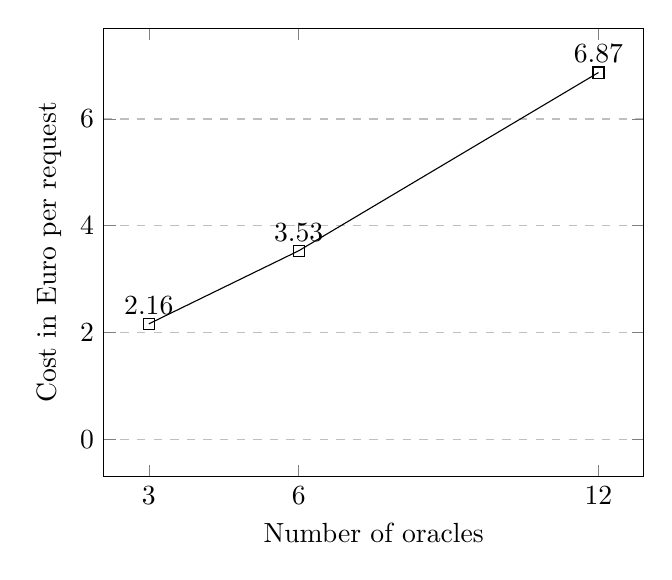
\begin{tikzpicture}
    \begin{axis}[
        xlabel={Number of oracles},
        ylabel={Cost in Euro per request},
        xtick=data,
        x tick label style={
            /pgf/number format/1000 sep=},
        xmin=3, xmax=12,
        ymin=0, ymax=7,
        ytick={0,2,4,6,8},
        ymajorgrids=true,
        grid style=dashed,
        enlargelimits=0.10,
      ]

      \addplot[
        mark=square, nodes near coords
      ]
      coordinates {
          (3,2.16)(6,3.53)(12,6.87)
        };

    \end{axis}
  \end{tikzpicture}
  \caption{Cost per query using a consensus of 2/3,}{Queried Google Finance on the 22th of May, 2019.}
  \
  \label{oracle-query-cost}
\end{figure}

\subsection{Component analysis}


\subsubsection{On-Chain Oracle}

The on-chain oracle is a smart contract that has an array which stores the requests made to the contract. Hard-coded in the contract is the predefined minimum quorum, which is the minimum number of equal answers needed to trust in the declaration of a final result. This minimum quorum will be used in all requests to the contract.
Also hard-coded are the white-listed addresses of oracles that the contract will accept transactions to update requests.

Initially the request structure \ref{code:request-struct} only contains the URL which will be queried by the off-chain oracle and the attribute to return in the json API response.

\begin{lstlisting}[language=Solidity, label=code:request-struct]
  struct Request {
    uint id;                            //request id
    string urlToQuery;                  //API url
    string attributeToFetch;            //json attribute (key) to retrieve in the response
    string agreedValue;                 //value from key
    mapping(uint => string) anwers;     //answers provided by the oracles
    mapping(address => uint) quorum;    //oracles which will query the answer (1=oracle hasn't voted, 2=oracle has voted)
  }
\end{lstlisting}


\subsection{Summary and Conclusions}
